\documentclass[../dissertation.tex]{subfiles}

\begin{document}

\section{Experiment 7 - Vertical Scaling}
\label{experiment7-vertical-scaling}

Prior experiments have been setting the groundwork for these scaling experiments. It is now understood how a communication intensive ROS application behaves in the simple case (2 hosts, 2 nodes), and how switching to a wireless network affects the performance.

Now we wish to understand how adding more communication nodes will affect individual message latency, and total system throughput in terms of messages sent.

This experiment will involve adding more nodes to both sender, and echoer. Each sender node will send messages to 1 echoer node, who will echo the message back to that same sender node. This allows the sender to record both sent and receive times consistently.

Increasing numbers of nodes will be added to each host, and message times recorded. The number of hosts will be a constant (2) as this experiment investigates the effect of increased ROS node counts only.

The data used will be the sensor data stream used in previous experiments.

\subsection{Results}

Figure \ref{exp7-100hz-allnodes} displays the averaged (across 3 runs) data for the 100Hz message frequency. This figure shows that performance degrades very rapidly for high node counts. At 100Hz using 8 total nodes (4 senders) results in poor performance with a message latency of 5 seconds by the end of the stream.

Figure \ref{exp7-100hz-lownodes} shows only the `good' performing node counts (1 and 2 senders) for a message frequency of 100Hz. There are apparent spikes in the message latency at regular intervals. One hypothesis for these spikes is that the senders are buffering messages, perhaps to allow other system processes to use the network interface. However, these spikes do not significantly affect the wider experiment, since they are only short lived spikes.

\begin{figure}[H]
\centering
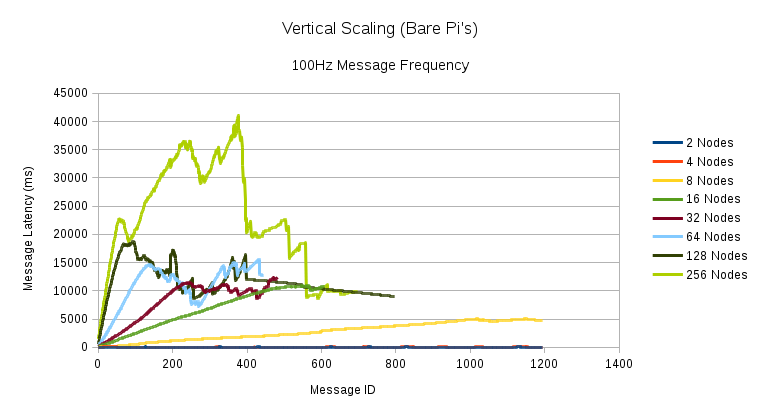
\includegraphics[width=\textwidth]{images/experiment7/vertical_scaling_100hz_all_node_counts.png}
\caption{Experiment 7 - 100Hz Message Frequency, All Node Counts}
\label{exp7-100hz-allnodes}
\end{figure}

\begin{figure}[H]
\centering
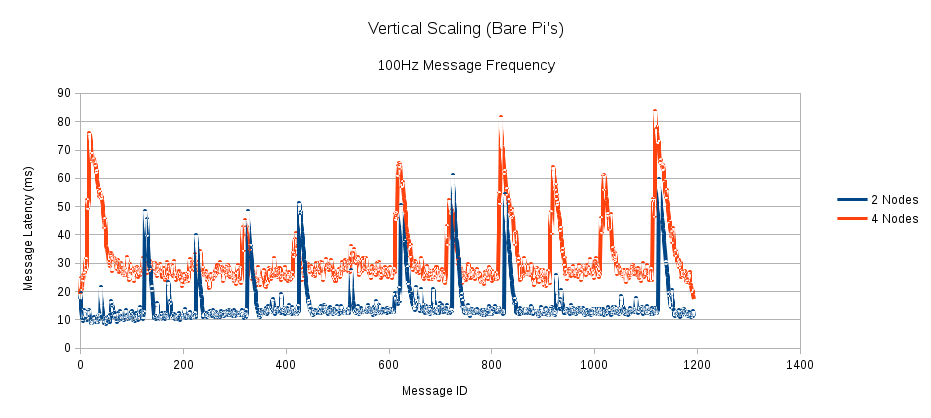
\includegraphics[width=\textwidth]{images/experiment7/vertical_scaling_100hz_low_node_counts.png}
\caption{Experiment 7 - 100Hz Message Frequency, Low Node Counts}
\label{exp7-100hz-lownodes}
\end{figure}

Figure \ref{exp7-200hz-allnodes} concerns a message frequency of 200Hz, and all node counts. This shows a similar pattern as Figure \ref{exp7-100hz-allnodes}, with a couple notable differences.

Perhaps most interesting is the behaviour of the 256 node (128 sender) case. As expected, performance is significantly worse at the start, peaking at a message latency of 50 seconds, however after this peak the performance begins to recover - finishing at similar performance levels as the 4 node (2 sender) case. The theorised cause behind this behaviour is that at such a high node count the host system locks up and ROS nodes begin dying. In this setup, there is no supervisor for the nodes so they are not restarted. Thus, if enough nodes die, the rest can continue functioning. This, however, is not useful behaviour in practise, as the system must halt for a long-enough time for the ROS Master's SSH connections to time out.

Another notable difference in the 200Hz case is that the 4 node (2 sender) case begins exhibiting degraded performance. This harkens back to results of Experiment 6 in Section \ref{experiment-6}, where a maximum frequency of greater than 300Hz began to show unsustainable performance.

\begin{figure}[H]
\centering
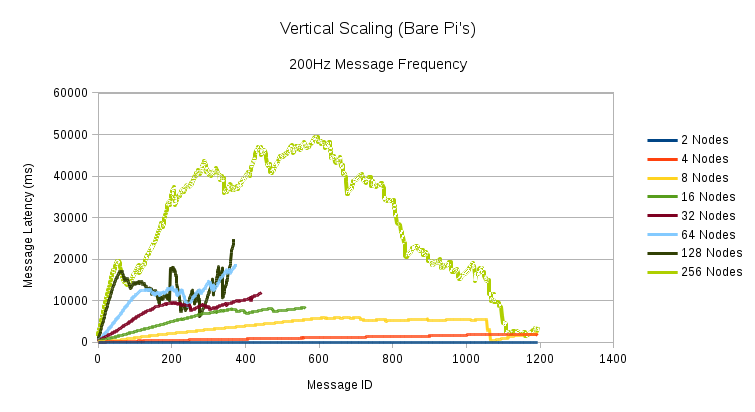
\includegraphics[width=\textwidth]{images/experiment7/vertical_scaling_200hz_all_node_counts.png}
\caption{Experiment 7 - 200Hz Message Frequency, All Node Counts}
\label{exp7-200hz-allnodes}
\end{figure}

Both of these observations hold for the 300Hz message frequency scenario, with more pronounced effects in both cases. From this data, we can see the system achieves good, sustainable performance with the following set-ups: 100Hz * 1 (sending) node, 100Hz * 2 nodes, 200Hz * 1 node, and 300Hz * 1 node.

From these observations we can conclude that the results of Section \ref{experiment-6} hold true in a more general sense, these results show that each host appears to have a communication scaling limit. This can be represented as the product of three quantites: the number of sending nodes on the host ($N$), the message frequency ($f_m$), and the message size ($S_m$) - giving the following equation for a Communication Scaling Limit Volume (CSLV):

\begin{center}
$CSLV = N \cdot f_m \cdot S_m$
\end{center}

Using this equation, we can calculate the CSLV for our particular platform (Raspberry Pi 3 Model B, running ROS Kinetic) using experimental data. However, in order to demonstrate the robustness of this hypothesis, further experiments in varying the $S_m$ (the message size) would be required.

\subsection{Further Investigation}

In order to get a clearer idea of how adding more ROS nodes affects the system, it is clear that we must use a lower message frequency which allows for sustainable performance at higher node counts.

Thus the above set-up was repeated, but with lower message frequencies. If the CSLV hypothesis were to hold true, we should be able to calculate which node counts will begin to show issues at each message frequency.

In this experiment, message frequencies of 1Hz, 10Hz, and 20Hz were used. Thus, at 1Hz we can expect greater than approximately (300Hz / 1Hz) 300 nodes to cause issues (we can ignore message size as we are using the same message size as previously). Respectively, we can expect the limit to lie around 30 nodes at 10Hz, and 15 nodes at 20Hz.

\begin{figure}[H]
\centering
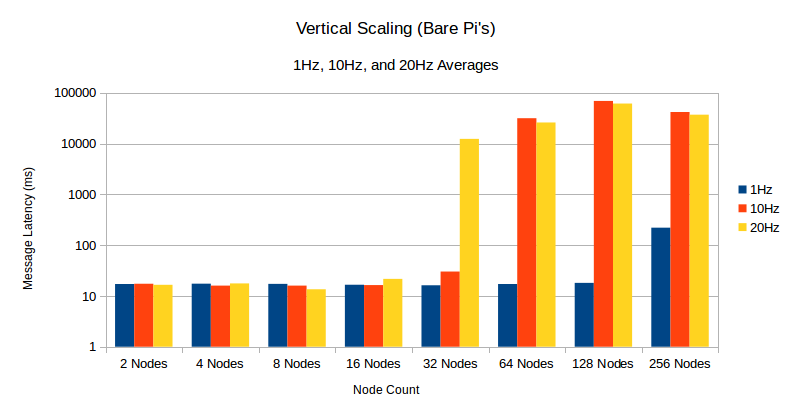
\includegraphics[width=\textwidth]{images/experiment8/vertical_scaling_all_freqs_log_avg_msg_latency.png}
\caption{Experiment 8 - Logarithmic Average Message Latency, All Frequencies, All Node Counts}
\label{exp8-all-freqs-averages}
\end{figure}

\textit{As Figure \ref{exp8-all-freqs-averages} shows (note the logarithmic latency scale), our expected supported node calculations were approximately correct, but somewhat underestimated the actual limits.} This under-estimation is expected, as the resolution of Experiment 6 was only 50Hz (300Hz was acceptable, 350Hz had poor performance), thus the true maximum is somewhere between 300Hz and 350Hz. The figure shows that performance was acceptable at $\leq$ 16 nodes at 20Hz, $\leq$ 32 nodes at 10Hz, and $\leq$ 256 nodes at 1Hz.

An data series of interest is that of 256 nodes at 1Hz message frequency. We can see in Figure \ref{exp8-1hz-all-nodes} the performance at this configuration is significantly worse than that at 128 nodes and less, but the performance was not as catastrophic as seen at all other frequencies (1Hz mean is 221ms, vs 10Hz mean of 41,895ms). Performance at this level was also somewhat consistent throughout the message stream, with most messages taking ~200ms RTT - again, unlike other message frequencies at 256 nodes. \textit{This indicates that a different bottleneck is possibly coming in to play. For example, perhaps the time spent switching processes contexts (between 256 different Python processes) is causing a consistent delay.} This reduced performance at 256 nodes was unexpected, according to the CSLV equation.

\begin{figure}[H]
\centering
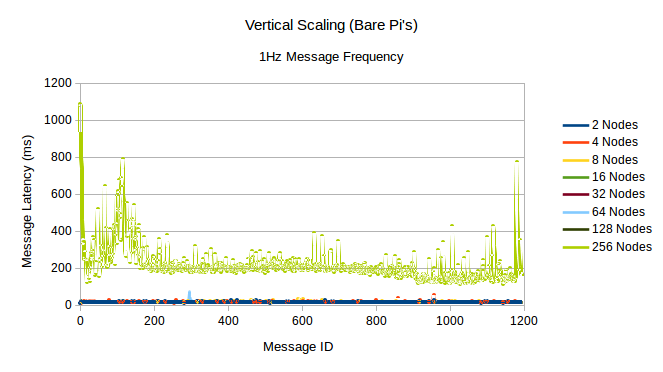
\includegraphics[width=\textwidth]{images/experiment8/vertical_scaling_1hz_all_node_counts.png}
\caption{Experiment 8 - 1Hz Message Frequency, All Node Counts}
\label{exp8-1hz-all-nodes}
\end{figure}



\end{document}
